\documentclass[border=6pt]{standalone}
\usepackage{amsmath,amssymb}
\usepackage{tikz}
\usetikzlibrary{shapes.geometric, arrows.meta, positioning, fit, calc}
\begin{document}
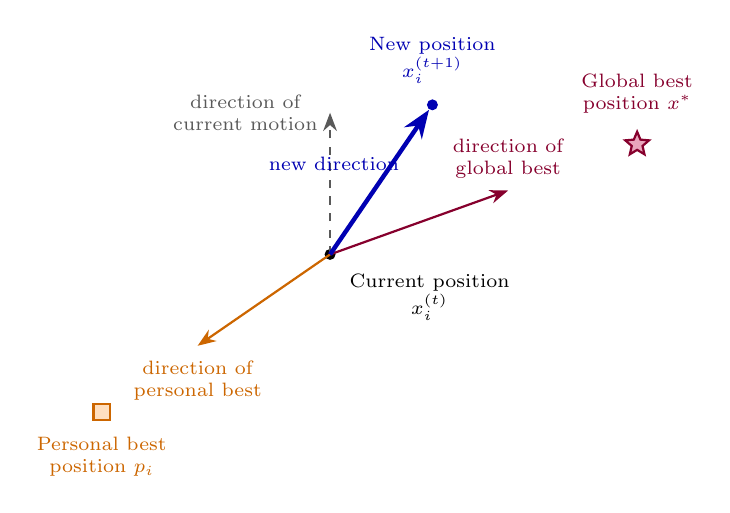
\begin{tikzpicture}[
    every node/.style={font=\scriptsize},
    ptmark/.style={circle, fill=black, inner sep=1.4pt},
    newmark/.style={circle, fill=blue!70!black, inner sep=1.4pt},
    pbestmark/.style={rectangle, draw=orange!80!black, fill=orange!25, line width=0.8pt, inner sep=1.5pt, minimum size=6pt},
    gbestmark/.style={star, star points=5, star point ratio=2.2, draw=purple!70!black, fill=purple!35, line width=0.8pt, inner sep=0.5pt, minimum size=9pt},
    inertiaarr/.style={-Stealth, thick, gray!70!black, dashed},
    cogarr/.style={-Stealth, thick, orange!80!black},
    socarr/.style={-Stealth, thick, purple!70!black},
    resarr/.style={-Stealth, ultra thick, blue!70!black}
]
\coordinate (Xt) at (0,0);
\coordinate (Pi) at (-2.9,-2.0);
\coordinate (G) at (3.9,1.4);
\coordinate (Xt1) at (1.3,1.9);

\node[pbestmark] (pbestpt) at (Pi) {};
\node[below=2pt of pbestpt, text=orange!80!black, align=center] {Personal best\\position $p_i$};

\node[gbestmark] (gbestpt) at (G) {};
\node[above=2pt of gbestpt, text=purple!70!black, align=center] {Global best\\position $x^{*}$};

\node[ptmark] (curpt) at (Xt) {};
\node[below right=2pt and 2pt of curpt, align=center] {Current position\\$x_i^{(t)}$};

\node[newmark] (newpt) at (Xt1) {};
\node[above=2pt of newpt, text=blue!70!black, align=center] {New position\\$x_i^{(t+1)}$};

\draw[inertiaarr] (Xt) -- (0,1.8) coordinate (inertiatip);
\node[left=1pt of inertiatip, text=gray!70!black, align=center] {direction of\\current motion};

\draw[cogarr] (Xt) -- ($(Xt)!0.58!(Pi)$) coordinate (cogtip);
\node[below=2pt of cogtip, text=orange!80!black, align=center] {direction of\\personal best};

\draw[socarr] (Xt) -- ($(Xt)!0.58!(G)$) coordinate (soctip);
\node[above=1pt of soctip, text=purple!70!black, align=center] {direction of\\global best};

\draw[resarr] (Xt) -- (newpt);
\node[text=blue!70!black] at (0.05,1.15) {new direction};
\end{tikzpicture}
\end{document}
